\documentclass[11pt]{article}

\usepackage[english]{babel}
\usepackage{amsmath}
\usepackage{amsfonts}
\usepackage{algpseudocode}
\usepackage[linesnumbered,ruled]{algorithm2e}
\usepackage[margin=2.5cm]{geometry}
\usepackage{graphicx}

\newcommand\mycommfont[1]{\footnotesize\ttfamily{#1}}
\SetCommentSty{mycommfont}

\newcommand\vect[1]{\boldsymbol{#1}}

\SetKwProg{Fn}{Function}{}{}
\SetKwRepeat{Do}{do}{while}
\SetKwRepeat{Do}{do}{while}
\SetKwBlock{Begin}{Begin:}{End}

\begin{document}
\begin{algorithm}[H]
\DontPrintSemicolon
	\caption{Generate random 3D trajectory (Initial basic version)}

	%\SetKwInOut{Input}{Input}
	%\SetKwInOut{Output}{Output}
	%\Input{Two nonnegative integers $a$ and $b$}
	%\Output{$\gcd(a,b)$}
	
	\SetKwInOut{Parameter}{Initialize}
	\Parameter{$a = 0.9, b = 1, \vect{x}_0 = (0,0,0), \vect{q}_0, \vect{v}_0 = (0,0,0)$ }
	\tcc{ $\vect{x}_0$ is the initial position vector, $\vect{q}_0$ is the quaternion describing initial orientation, and  $\vect{v}_0$ is the initial velocity vector}
	
	%\Begin{
		\For{$t \gets 0$ \KwTo $T$}{
			
			\If{check for obstacles on line: $\vect{x}_t + \alpha \vect{v}_t$ is true}{ 
				\tcc{$\alpha > 0$ tells the look ahead distance}
				\tcc{change heading or velocity slightly towards better direction}
				
				$\vect{v} \gets \vect{v}_t$ \;
				\While{check for obstacles on line: $\vect{x}_t + \alpha \vect{v}$ is true}{
					$ \zeta \sim \mathcal{N}( \vect{\mu},\,\vect{\Sigma}) $ \;
					$\vect{v} \gets a \vect{v}_{t-1} + b \zeta $ \;
					\tcc{note: $\vect{v}$ is just a temporary velocity variable until we find a better direction}
				}
				$\vect{v}_t \gets \vect{v}$
			}\;
			
			$\vect{x}_{t+1} \gets \vect{x}_t + \vect{v}_t $ \;
			\tcc{sample $\eta$ from multivariate (3 dimensional) standard normal distribution}
			$ \eta \sim \mathcal{N}( \vect{\mu},\,\vect{\Sigma}) $ \;
			%\tcp*[l]{sample $\eta$ from multivariate (3 dimensional) standard normal distribution}
			$\vect{v}_{t+1} \gets  a \vect{v}_t + b \eta $ \;
			
			\tcc{Quaternion orientation is not required for initial version}
			\tcc{ can skip this update}
			$ \vect{q}_{t+1} \gets  \sf{FindQuaternion}(\vect{v}, \mathbf{y}_{world}) $ 
		}\;
	%} \;
	\Fn{ \sf{FindQuaternion ($\vect{v}$, $\mathbf{y}_{world}$)} }{
	\tcc{assumes our heading in always along y axis of \lq body\rq \ frame }
	Normalize $\vect{v}$ to unit vector $\vect{\hat{v}}$ \;
	$\theta \gets \arccos (\vect{\hat{v}} \cdot \vect{y}_{world})$ \;
	$\vect{\hat{u}} \gets (\vect{\hat{v}} \times \vect{y}_{world})$ \;
	 $\vect{q} = (\ \cos(\frac{\theta}{2}), \ \sin(\frac{\theta}{2}) \ \vect{\hat{u}} \ ) $\;
	 \Return $\vect{q}$
	}
\end{algorithm} 

Sample trajectory (below)

\begin{figure}[h]
	\centering
	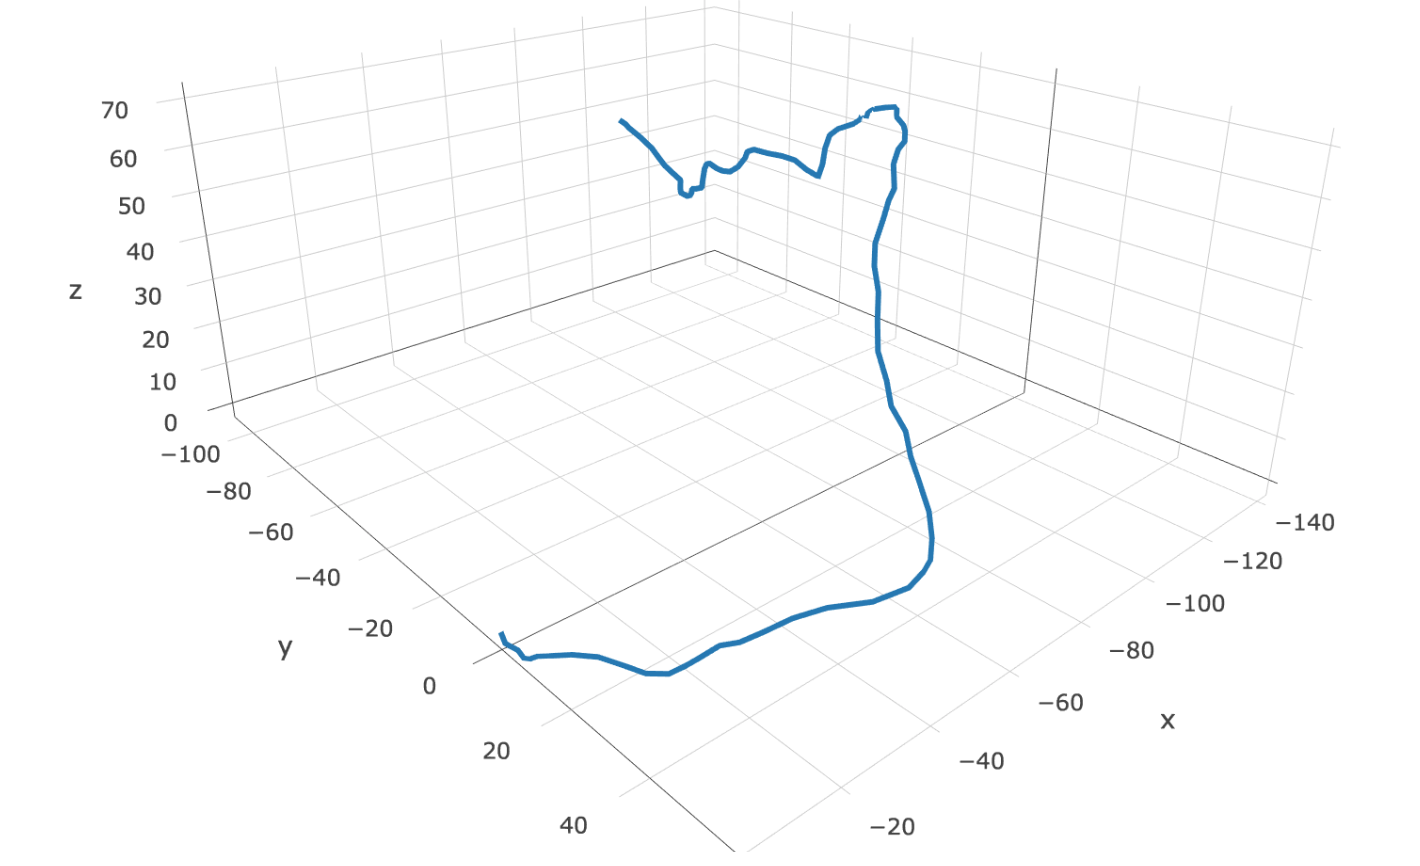
\includegraphics[width=0.8\textwidth]{3d}
        \caption{Sample 3D trajectory generated by above algorithm (without quaternions)}
        \label{3d}
\end{figure}

\end{document}